\chapter{MCU}
\label{chap:MCU}
Im Projekt 5 wurde bereits eine MCU ausgewählt, mit der das Prototyping erfolgte. Aufgrund der Verfügbarkeit (bei der FHNW bezugsbereit) wurde ein Arduino Mega2560 Board verwendet. Auf den kommenden Abschnitt aus dem Fachbericht des Projekt 5 folgt ein Abschnitt mit ergänzenden Informationen aus der Bachelor-Thesis.

\section{MCU - Projekt 5}
Die Micro Controller Unit (MCU) ist der zentrale Bestandteil für die Kommunikation, resp. für den Datenaustausch zwischen den unterschiedlichen Modulen. Sie interpretiert die Signale der Sensoren und rechnet sie in die interessierenden Messwerte um. Dann weist die MCU jedem Messwert einen Zeitstempel über das RTC zu und übergibt diesen der Datenspeicherung. Wenn die Daten vom Kommunikationsmodul angefordert werden, liest die MCU die Datenspeicherung aus und übergibt sie dem Kommunikationsmodul.\\

{\begin{minipage}[b][130pt][t]{0.5\textwidth}
Für die Entwicklung der MCU wird ein Arduino Mega Board verwendet. Der Vorteil besteht darin, dass elementare Bauteile (Hardware) bereits implementiert sind, wie z.B. Oszillator, der USB-Anschluss und die PCB-Connectors für ein schnelles Prototyping. Die wichtigsten technischen Daten sind in der Tabelle \ref{tab:arduinoMega_technischeDaten} aufgelistet.\\
\end{minipage}}
\hfill
{\begin{minipage}[b][130pt][t]{0.49\textwidth}
\centering
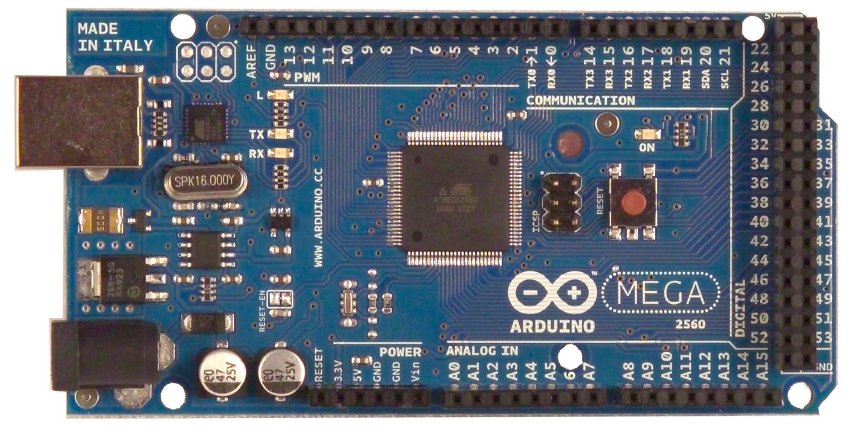
\includegraphics[width=0.99\textwidth]{graphics/MCU/arduino_mega.png}
\captionof{figure}{Arduino Mega Board \cite[S.1]{arduinoMega}}
\label{fig:arduinoMega}
\end{minipage}}

\begin{table}[h]
\centering
\caption{Technische Daten \cite[S.3]{arduinoMega}}
\begin{tabular}{|l|l|}
\hline 
Microcontroller & ATmega2560 \\ 
\hline 
Operating Voltage & 5V \\ 
\hline 
Digital I/O Pins & 54  \\ 
\hline 
Analog Input Pins & 16 \\ 
\hline 
Flash Memory & 256 KB, 8 KB werden vom bootloader benötigt\\ 
\hline 
SRAM & 8 KB \\ 
\hline 
EEPROM & 4 KB \\ 
\hline 
Clock Speed & 16 MHz \\ 
\hline 
\end{tabular}
\label{tab:arduinoMega_technischeDaten}
\end{table}

\section{Ergänzungen aus der Bachelor-Thesis}
Während der Bachelor-Thesis kam die Idee auf, eine kleinere MCU zu verwenden. Eine kleinere MCU hat die Vorteile, dass diese günstiger ist in der Anschaffung, einen geringeren Stromverbrauch aufweist und weniger Platz auf dem PCB benötigt.  Aufgrund der Firmware wird jedoch eine erhöhte Menge Speicher alloziert, weshalb die \textit{Data Memory Usage} des verwendeten ATMega328 zu klein war und wieder auf den bereits für das Prototyping verwendeten ATMega2560 zurückgegriffen werden musste. \\
